\section{Design Limitations}
The working setup that exists at Aalborg University (AAU) is composed by one of the sides of the 3D cube.

Since all the hardware is already build, the goal of the project is focus on deriving the model of the system, simulate it to compare it with the real Cubli and design a controller capable of balance it in the equilibrium position.

One important characteristic is that one of its corners is attached to a base plate. This feature limits the number of movements the Cubli can do, as it can only be balance in one direction.

Another important limitation is given by the maximum current that the motor can provide which conditions the maximum starting angle that it can have with respect to equilibrium position. As can be seen in \figref{}, if the initial angle is different from 0 rad both the mass of the frame ans the mass of the wheel exert an initial torque to the system. This must be overcame by the motor in order to the Cubli not to fall.
%
\begin{figure}[H] 
	\centering
	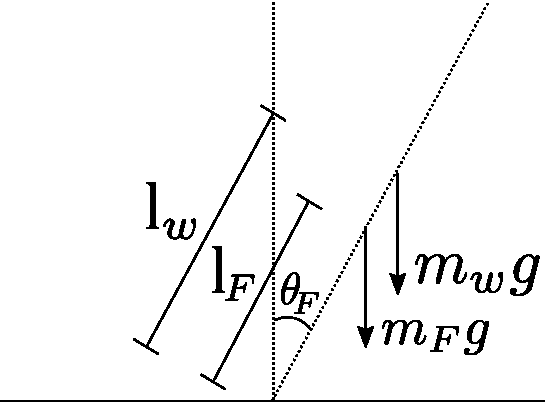
\includegraphics[scale=0.65]{figures/limitationTorque}
	\caption{Force acting on the system that create an initial torque}
	\label{limitationTorque}
\end{figure}

The minimum torque that the motor must apply is give by \eqref{minTorque}.
%
\begin{flalign}
	\eq{T} { (m_F \cdot l_F + m_w \cdot l_w) \cdot g \cdot sin(\theta_F)} \unit{N\cdot m}
	\label{minTorque}
\end{flalign}

Since the torque is restricted by the characteristics of the motor and the control board, the maximum initial angle is derived in \eqref{maxAngle}.
%
\begin{flalign}
	\eq{\theta_F} { asin\left(\frac{T}{(m_F \cdot l_F + m_w \cdot l_w) \cdot g}\right)} \unit{N\cdot m}
	\label{maxAngle}
\end{flalign}
%
Substituding the values of the maximum torque (see section \ref{sec:Motor}) and the parameters of the Cubli (see section \ref{sec:Param}) the maximum starting angle is \si{0,2024\ rad}.

\fxnote{The maximum angle may should be explained after the modeling and the estimation of parameters}
%At Aalborg University (AAU), there exists a working setup of a one-dimensional Cubli. The overall goals of this semester are to make a model of a system, to simulate this model and then to design and implement a controller for that system. Students on this semester are encouraged to work with pre-made setups, since the focus is rather on the control engineering than the hardware solution.\fxnote{moved the section directly from introduction. Will need a top to catch the previous chapter}

